% -*- mode:flyspell; mode:latex  -*-

%%% Local Variables:
%%% TeX-master: "mu2e-36575"
%%% End:

%%%%%%%%%%%%%%%%%%%%%%%%%%%%%%%%%%%%%%%%%%%%%%%%%%%%%%%%%%%%%%%%%%%%%%%%%%%%% 
\section{Track quality selections}
{\blue lowercase title words after first word}

%%%%%%%%%%%%%%%%%%%%%%%%%%%%%%%%%%%%%%%%%%%%%%%%%%%%%%%%%%%%%%%%%%%%%%%%%%%%%%
\subsection{\MuToEm\  channel}
\label{sec:mumem_channel}
{\blue lowercase title words after first word}

Selection of correctly reconstructed tracks plays a critical role in the search, and 
to improve rejection of poorly reconstructed  tracks, an MVA-based technique is used.
A MLP ANN is trained to distinguish between correctly reconstructed tracks
and mis-reconstructed ones\strike{,}{\blue ;} good tracks are selected by requiring the ANN 
score to be above {\blue a} certain value.

In the Mu2e offline, \strike{two different track fits are}
{\blue there are two different track fits} used to determine the track parameters.
Both \strike{are using} {\blue fits use} the same fitting algorithm, but the fits are 
performed with two different hit ambiguity resolvers\strike{,}{\blue -} a panel-based ambiguity 
resolver\strike{, or PAR,} {\blue (PAR)} and a doublet-based ambiguity resolver\strike{, or DAR}
{\blue (DAR)}. A track quality ANN has been trained only for one of them,
the PAR{\blue , in the current version of the Mu2e Offline}. 
%
We performed a similar training for the output of the DAR track fits.
%
Following \cite{MU2E_4595_ANN_TRAINING}, we used {\blue the} ROOT TMVA package to train a{\blue n}
MLP ANN with 8 input variables and one hidden layer. The following eight variables were used
as inputs:

\begin{itemize}
\item
  {\bf na } : {\blue the} number of \strike{``active''} {\blue active} hits remaining on the track
  after the Kalman fit and used in the calculation of the fit $\chi^2$
\item
  {\bf nafract} : \strike{na/nhits , a} {\blue the} ratio of the number of active hits to the total number
  of hits (after the seed fit)
\item
  ${\bf \strike{log_{10}{fcons}} {\blue log_{10}(fcons)}}$ : {\bf fcons}, or {\blue the} fit consistency{\blue ,}
  is a probability-minded derivative \strike{from} {\blue of} the track fit $\chi^2$. {\blue The l}\strike{L}ogarithm
  of it is taken \strike{from the} {\blue for} numerical considerations
\item
  {\bf momerr} : {\blue the} uncertainty on the reconstructed track momentum, returned by the fitter
\item
  {\bf t0err} : {\blue the} uncertainty on the reconstructed track time, \strike{T0} {\blue $T_0$}, returned by the fitter
\item
  {\bf fda} : \strike{Nd/Na,} {\blue the} fraction of \strike{``doublet''} {\blue doublet} active hits {\blue over total number of active hits}
\item
  {\bf fza } : \strike{Nza/Na,} {\blue the} fraction of active\strike{v} hits with undefined drift direction
\item
  {\bf fma } : {\bf \red to be clarified}
\end{itemize}

The ANN training is aimed to optimize the separation of electron tracks reconstructed correctly, 
\strike{with} {\blue defined as} ${\blue |}\Delta{P} {\blue |}= |P_{reco}-P_{true}| < 0.25$ MeV/c, or approximately within 
$2\sigma$ \strike{from} {\blue of} the true value, from tracks
{\blue with significantly larger reconstructed momentum, defined as}
\strike{reconstructed with} $\Delta{P} > 0.7$ MeV/c, \strike{or , approximately,} {\blue or approximately} $5\sigma$
above the true value.
\strike{\textbackslash n}
Comparison between $P_{true}$ and $P_{reco}$ was performed in a plane corresponding to the
tracker front.
%
\strike{Used for the ANN training were tracks with |D0| < 100 mm and 0.5 < \tandip < 1.}
{\blue Tracks with |D0| < 100 mm and 0.5 < \tandip < 1 were used to train the ANN.}

To choose between the PAR-based and DAR-based fitters, we compared performance of the
trained DAR ANN to the performance of the default for the \strike{offline} {\blue Mu2e Offline} v9\_0\_5 \strike{offline} PAR ANN.
%
\strike{Using the CD3 choice of the signal region , 103.85 < P < 104.90 MeV/c, $T_0 > 700$ ns, we compared performances of the two methods.}
{\blue We compared the performance of the two methods using the CD3 choice for the signal region: 103.85 < P < 104.90 MeV/c and $T_0 > 700$ ns.}
%
Figure \ref{fig:mumem_ann_operational_point_choice} shows the expected DIO background plotted
versus the CE reconstruction efficiency. Both are plotted in relative units, normalized
to the DIO background and CE efficiency of the PAR track selection with the default
cut on the ANN score $S_{PAR} > 0.8$ \strike{respectively}.
%
\strike{Squares} {\blue Square markers} represent {\blue the} PAR track selection\strike{, circles -}
{\blue and circle markers repesent the} DAR track selection\strike{,}{\blue ;} red and black colors
correspond to the \strike{CE+1} {\blue conversion electron signal MC with 1 and 2} batch mode pileup
\strike{and CE+2 batch mode} datasets \strike{correspondingly} {\blue respectively}.
%
In all cases the background model comes from the DIO-weighted fele2s51b1 dataset -
\strike{electrons +} {\blue flat energy electron MC with} 1 batch {\blue mode} pileup. 

As follows from Figure \ref{fig:mumem_ann_operational_point_choice}, \strike{for the same expected 
background level, using the DAR tracks allows to increase acceptance by 4-5\%.}
{\blue using the DAR tracks increases the signal acceptance by 4-5\% with respect to PAR tracks for the same expected  background level.}
One can also see, that the {\blue Mu2e Offline default} choice of the PAR ANN operational point is quite close to the optimum - after the 
(1,1) point the PAR background starts increasing much faster than the PAR signal,
and the increase by 5\% comes along with \strike{the} {\blue a} x2 higher DIO background.

For the DAR tracks, improving the signal acceptance by the same 5\% \strike{wrt} {\blue with respect to} the default \strike{offline}
{\blue Offline} selection \strike{doesn't} {\blue does not} cost extra background. This determines the choices for {\blue the} SU2020 analyses: 

\begin{itemize}
\item
  SU2020 analyses use DAR tracks
\item
  the ANN operational point corresponds to the cut on the output of $S_{DAR} > 0.2$.
\end{itemize}

\begin{figure}[H]
\begin{tikzpicture}
  \node[anchor=south west,inner sep=0] at (0,0.) {
    % \node[shift={(0 cm,0.cm)},inner sep=0,rotate={90}] at (0,0) {}
    \makebox[\textwidth][c] {
      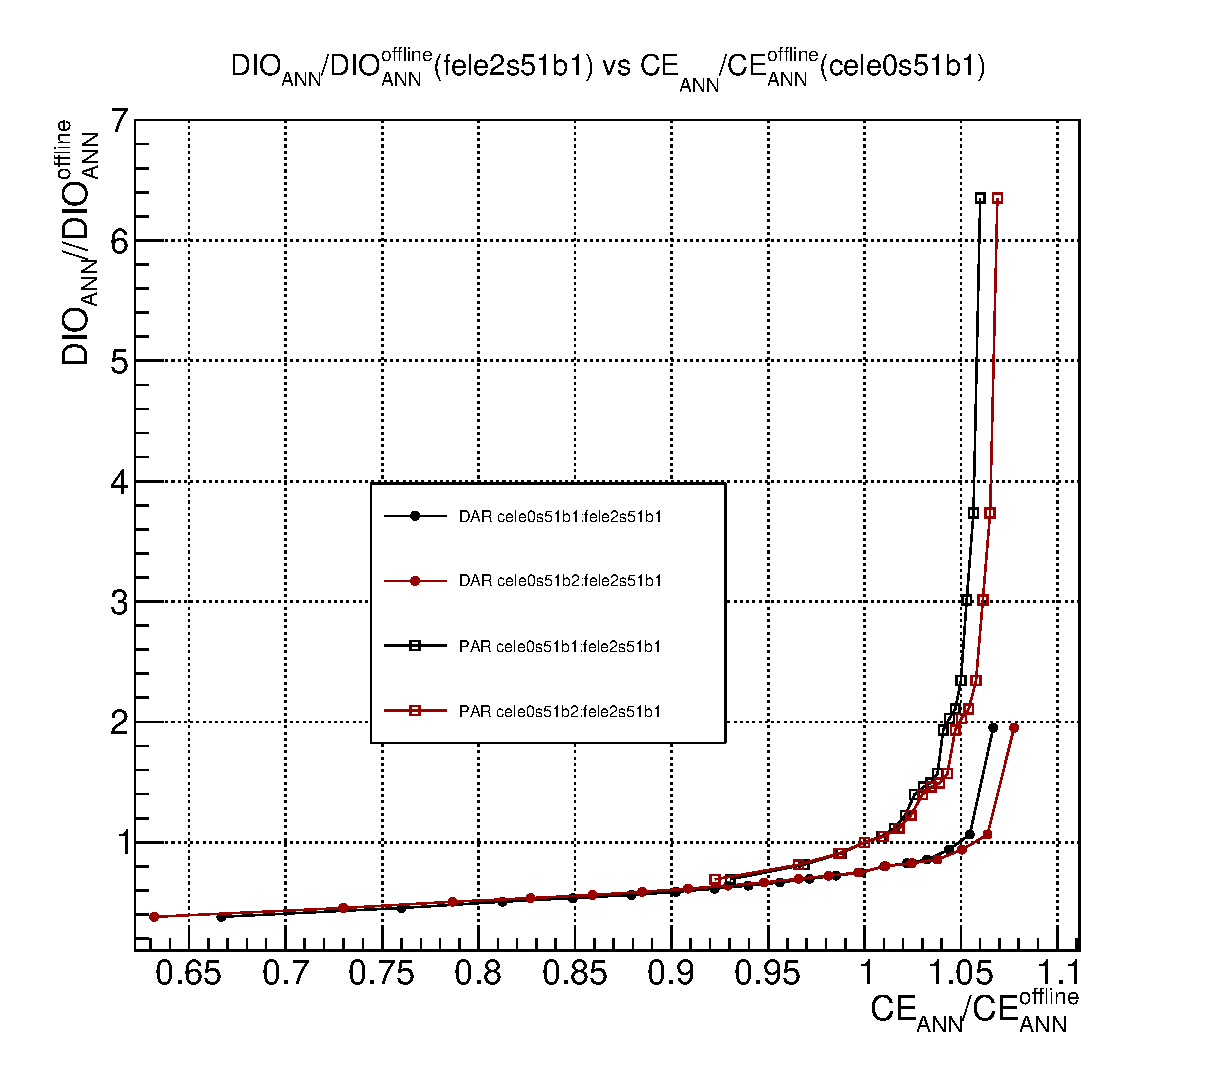
\includegraphics[width=0.8\textwidth]{figures/pdf/mumem_trq_ann_signal_vs_background}
    }
  };
  % \node [text width=6cm, scale=0.8] at (4.5,6.4) {mu2e-18894 by Kevin Lynch and Jim Popp};
\end{tikzpicture}
% \captionof{figure} {
\caption{
  \label{fig:mumem_ann_operational_point_choice}
  \strike{Choice of the ANN operational point.} {\blue Relative DIO background versus relative signal acceptance.}
  {\blue The e}\strike{E}xpected DIO background, \strike{in units of} {\blue relative to} the DIO background \strike{corresponding to} {\blue using the}
  default \strike{offline} {\blue Offline} PAR ANN track selection, is plotted versus efficiency \strike{for CE} 
  {\blue of the conversion electron signal acceptance}, normalized to the efficiency
  of the \strike{CE signal selection with the} {\blue signal using the default Offline} PAR ANN. 
  PAR curves go through \strike{(1,1) point} {\blue the point (1,1)} by construction.
  Background : DIO-weighted {\bf fele2s51b1}, \strike{CE} signal: {\bf cele0s51b1} (red), or {\bf cele0s61b2} (black).
  {\blue Default Offline} PAR track selection {\blue uses} $S_{PAR} > 0.8$;  \strike{DAR track selection: $S_{DAR} > 0.2$}
  {\blue where is this on the plot and how is it used? This seems to be a result from it, in which case it can be omitted here as it is in the note body.}
  \strike{Use of the DAR tracks instead of the PAR ones improves CE signal acceptance in the CD3 signal region of [103.85,104.90]
  by 4-5\%, while the corresponding DIO background is kept at a lower level} {\blue this is more interpretation repeated from the note body}
}
\end{figure}

Figure \ref{fig:mumem_dar_vs_par_ann} compares the track momentum resolution distributions 
for DAR and PAR tracks reconstructed in {\blue the 2 batch mode signal, }{\bf cele0s61b2}{\blue ,} dataset
\strike{and selected with different cuts on the corresponding ANN score.} {\blue using either a fixed background
or a fixed signal efficiency operational point.}\strike{\textbackslash n}
In Figure \ref{fig:mumem_dar_vs_par_ann}(a){\blue ,} the operational points for {\blue the} DAR and PAR track selection{\blue s}
are chosen to give the same expected background\strike{,}{\blue -} in Figure \ref{fig:mumem_dar_vs_par_ann}(b) \strike{-}{\blue ,}
the same track selection efficiency. {\blue A h}\strike{H}igher high-momentum tail in the distribution for PAR
tracks is clearly visible {\blue in both operational points}.

\begin{figure}
\hspace{-0.6in}
\begin{tikzpicture}
  \node[anchor=south west,inner sep=0] at (0,0.) {
    % \node[shift={(0 cm,0.cm)},inner sep=0,rotate={90}] at (0,0) {}
    % \makebox[\textwidth][c] {
    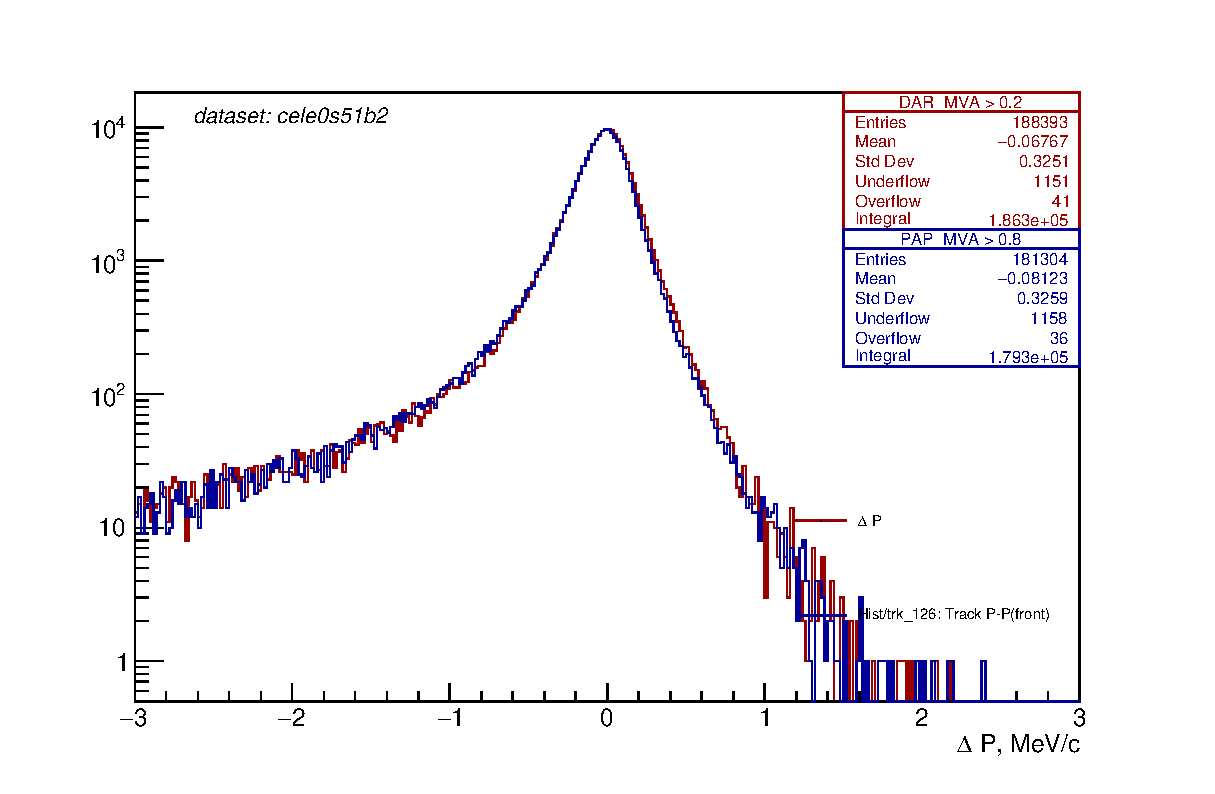
\includegraphics[width=0.64\textwidth]{figures/pdf/figure_00114_cele0s51b2_track_comp_ffff_1070_trk_214_vs_126_dpf}
    % }
  };
  \node [text width=1cm, scale=0.8] at (3.,4.5) {(a)};
  \node[anchor=south west,inner sep=0] at (10.5,0.) {
    % \node[shift={(0 cm,0.cm)},inner sep=0,rotate={90}] at (0,0) {}
    % \makebox[\textwidth][c] {
    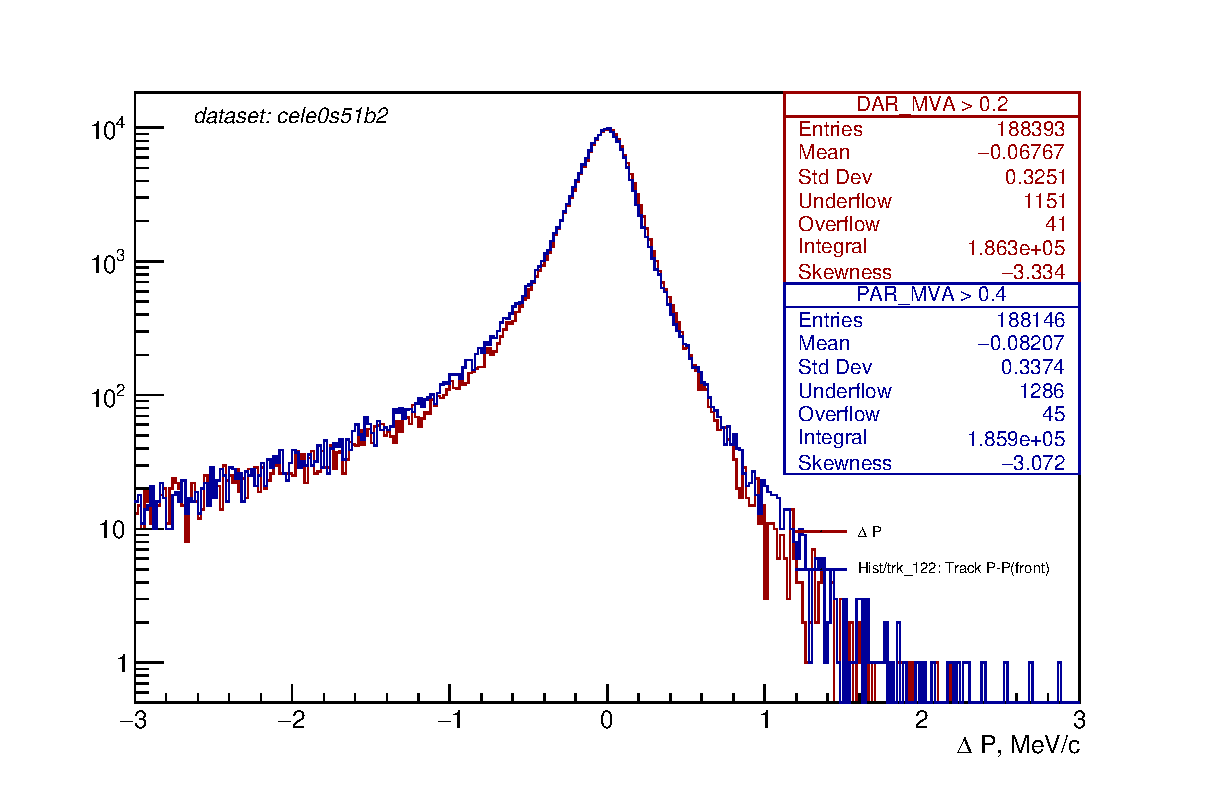
\includegraphics[width=0.64\textwidth]{figures/pdf/figure_00116_cele0s51b2_track_comp_ffff_1070_trk_214_vs_122_dpf}
    % }
  };
  \node [text width=1cm, scale=0.8] at (13.5,4.5) {(b)};
\end{tikzpicture}
% \captionof{figure} {
\caption{
  \label{fig:mumem_dar_vs_par_ann}
  DAR vs PAR track selection efficiency for two operational points: 
  (a): DAR and PAR selections correspond to the same background,{\blue is this the background level for the Offline default or the new working point (looks like the latter)?}
  (b): DAR and PAR selections correspond
  to the same efficiency. {\blue same question for what efficiency is used}  \\
  The right-side tail, \strike{determined by the misreconstructed} {\blue the most severely mis-reconstructed} tracks, is a measure of
  the track selection quality{\blue .} {\blue Legend should refer to lines as DAR or PAR; Left stats box should be PAR not DAP}
}
\end{figure}

Improvements in the track reconstruction, for the same selection efficiency, result in \strike{a significantly better
rejection of the misreconstructed tracks} {\blue significantly improved rejection of mis-reconstructed tracks}.
Figure \ref{fig:dio_delta_p_1036_1050} shows the $\Delta{P}$ distribution
for the simulated DIO electrons (DIO-weighted \strike{fele2s51b1} {\blue \bf fele2s51b1}) with \strike{the} reconstructed track
\strike{momenta} {\blue momentum}
in [103.6, 105.0] MeV/c. From that distribution one can easily \strike{quantify} {\blue see the} importance of the relative contribution
of tracks with $\Delta{P}$ above {\blue a} certain threshold. In particular, tracks with significantly mis-reconstructed
\strike{momenta} {\blue momentum}, $\Delta{P} > 0.5$ MeV, represent about 0.23 of the expected DIO background
\strike{, about 50\% lower than 0.355, estimated for the same momentum window in \cite{MU2E_4595_ANN_TRAINING}..}
{\blue (which is about 50\% lower than the previous estimate of 0.355 for the same momentum window in \cite{MU2E_4595_ANN_TRAINING}).}

\begin{figure}
  \begin{tikzpicture}
    \node[anchor=south west,inner sep=0] at (0,0.) {
      % \node[shift={(0 cm,0.cm)},inner sep=0,rotate={90}] at (0,0) {}
      \makebox[\textwidth][c] {
        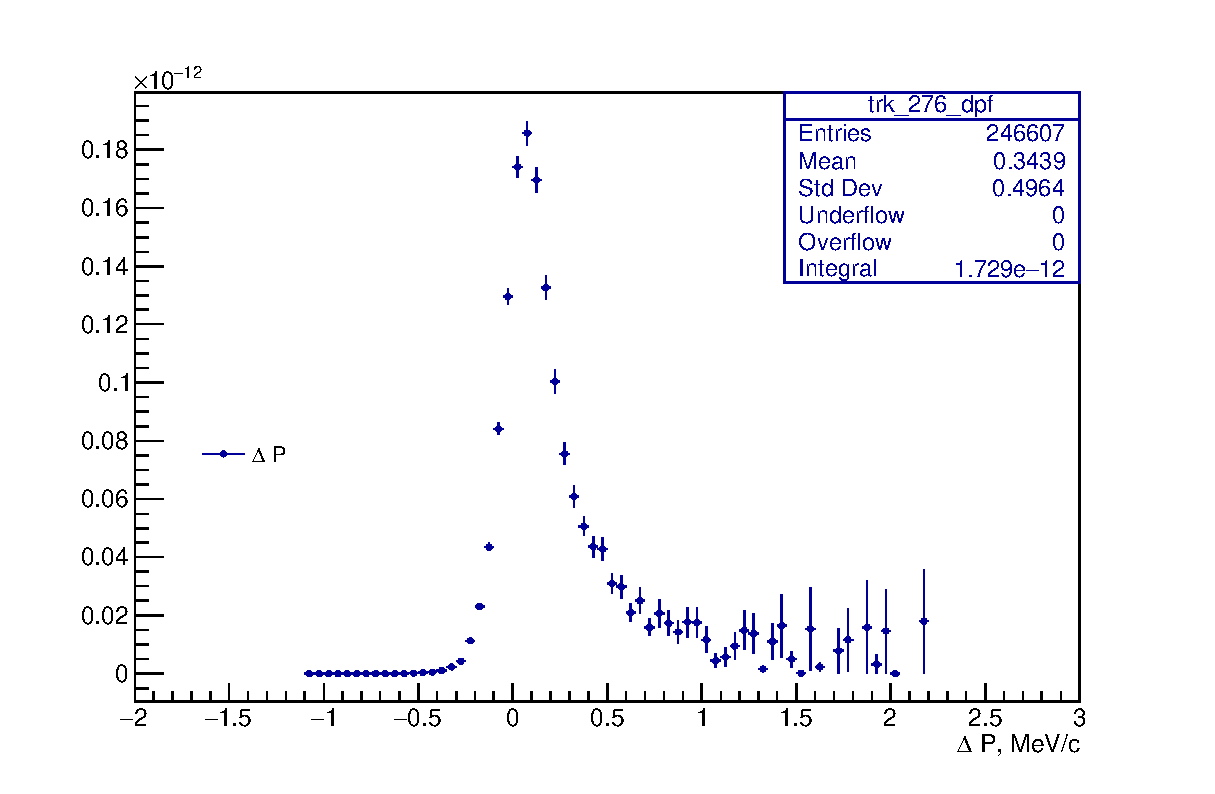
\includegraphics[width=0.99\textwidth]{figures/pdf/figure_00111_fele2s51b1_track_comp_ffff_1070_trk_276_dpf}
      }
    };
    % \node [text width=6cm, scale=0.8] at (4.5,6.4) {mu2e-18894 by Kevin Lynch and Jim Popp};
  \end{tikzpicture}
  % \captionof{figure} {
  \caption{
    \label{fig:dio_delta_p_1036_1050} 
    $\Delta P ~=~ P_{reco} -P_{true}$ distribution for {\blue the} simulated DIO background in the region [103.6,105.0] MeV.
    77.2\% of {\blue the} reconstructed events in this region are expected to have $\Delta P < 0.5$ MeV/c
  }
\end{figure}

As a cross-check, we used the TMVA package to train a BDT-based track quality classifier.
Similar to \cite{MU2E_33150_ANN_TRAINING}, we found that the MLP ANN performed slightly better,
so \strike{current analysis uses} {\blue current analyses use or the current analysis uses} a MLP ANN-based track quality selection.
\strike{\textbackslash n}
To explore the parameter space, the definition of a ``mis-reconstructed track'' has been varied and
a similar ANN has been trained to discriminate tracks reconstructed with $\Delta{P} < 0.25$ MeV/c {\blue is this $|\Delta{P}|$?}
from tracks with $\Delta{P} > 0.6$ MeV/c. No improvement in the DIO
suppression in the region [103.85, 104.9] MeV/c was observed. 

%%%%%%%%%%%%%%%%%%%%%%%%%%%%%%%%%%%%%%%%%%%%%%%%%%%%%%%%%%%%%%%%%%%%%%%%%%%%%%
\newpage
\subsection{\MuToEp\ channel}
\label{sec:mumep_channel}
{\blue lowercase title words after first word}

To select tracks in {\blue the} \MuToEp\ channel, a \strike{e+ + 1-batch} {\blue conversion positron MC with 1 batch}
mode pileup \strike{({\bf cpos0s51b1}) dataset } {\blue dataset ({\bf cpos0s51b1})}
has been used to train \strike{a} {\blue an} MLP ANN to discriminate between \strike{correctly} {\blue well reconstructed}
and mis-reconstructed positron tracks.
The ANN configuration and the definitions of \strike{a} well reconstructed and mis-reconstructed tracks are
the same as described in Section \ref{sec:mumem_channel}.

Figure \ref{fig:mumep_trq_ann} compares the expected background vs the signal efficiency curves,
\strike{in relative scale} {\blue relative to the default Offline positron selection (as in Figure \ref{fig:mumem_ann_operational_point_choice})},
for PAR (squares) and DAR {\blue (}circles) tracks.
\strike{As in Figure \ref{fig:mumem_ann_operational_point_choice}, the expected background and the signal
efficiency are plotted relative to the background and signal efficiency expected for the default
positive track selection implemented in offline v9\_0\_5.}
The background definition, however, is different. Unlike in \MuToEm\ channel, in \MuToEp\ there is
no well defined background process \strike{which} {\blue whose} contribution could be used as a measure of mis-reconstruction.
The RMC contribution depends on the assumptions about the RMC photon momentum distribution and,
in particular, its endpoint. Because of this, the background in Figure \strike{\ref{fig:mumem_ann_operational_point_choice}}
{\blue \ref{fig:mumep_trq_ann}}
is defined as the expected number of events with \strike{the misreconstructed} {\blue mis-reconstructed} momentum $\Delta{P} > 1.0$ MeV.
The signal is integrated over the [90.5,92.5] MeV/c momentum window\strike{,}{\blue .}

Figure \strike{\ref{fig:mumem_ann_operational_point_choice}}{\blue \ref{fig:mumep_trq_ann}}.(b) shows the same performance curves
as \strike{\ref{fig:mumem_ann_operational_point_choice}}{\blue \ref{fig:mumep_trq_ann}}.(a), but with the vertical axis in logarithmic scale.
It is interesting to see\strike{,} that for {\blue a} given background definition, the background increases exponentially
with the signal acceptance for both types of tracks.
\strike{\textbackslash n}
For the same signal acceptance, the ANN-based selection of DAR tracks results in lower
background{\blue s}, so the sensitivity estimate in \MuToEp\ channel also uses the DAR tracks. 

\strike{At to} {\blue For} the choice of the operational point, {\blue the} cut $S_{DAR} > 0.2$ improves the signal acceptance
by 10\%, while increasing the background by 15\%. Relaxing the cut and moving the cut value
to $S_{DAR} > 0.15$ adds another 2\% to the CP acceptance, while the background grows much faster
and becomes $B_{DAR}/B_{PAR}^{default} = 1.5,$
Thus, the default cut on \strike{the $S_{DAR}^-$} {\blue $S_{DAR}^+$} is the same as in the electron channel:  $S_{DAR}^- > 0.2$

An attempt to train a similar ANN for PAR tracks, somewhat surprisingly, didn't improve the performance
of the ANN-based PAR track selection, leaving a potential for further improvements. 
{\blue Clarify how the former trained ANN differs from the latter, as it's not clear why it should be different}

\begin{figure}[H]
  \hspace{-0.6in}
  \begin{tikzpicture}
    \node[anchor=south west,inner sep=0] at (0,0.) {
      % \node[shift={(0 cm,0.cm)},inner sep=0,rotate={90}] at (0,0) {}
      % \makebox[\textwidth][c] {
      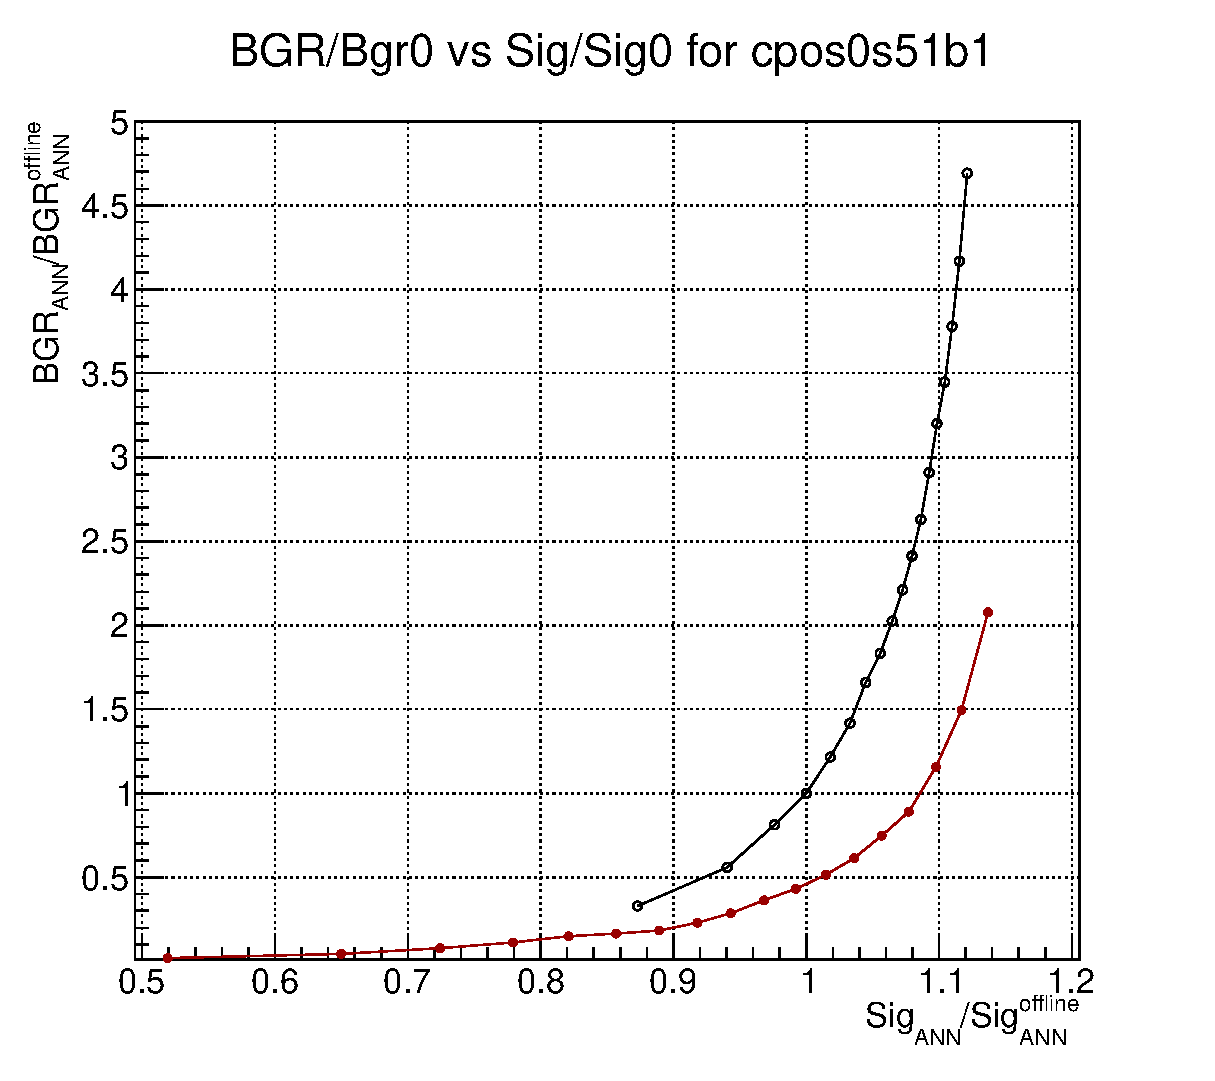
\includegraphics[width=0.55\textwidth]{figures/pdf/mumep_trq_ann_signal_vs_background_lin}
      % }
    };
    \node [text width=1cm, scale=1.0] at (3.,3.5) {(a)};
    \node[anchor=south west,inner sep=0] at (10,0.) {
      % \node[shift={(0 cm,0.cm)},inner sep=0,rotate={90}] at (0,0) {}
      % \makebox[\textwidth][c] {
      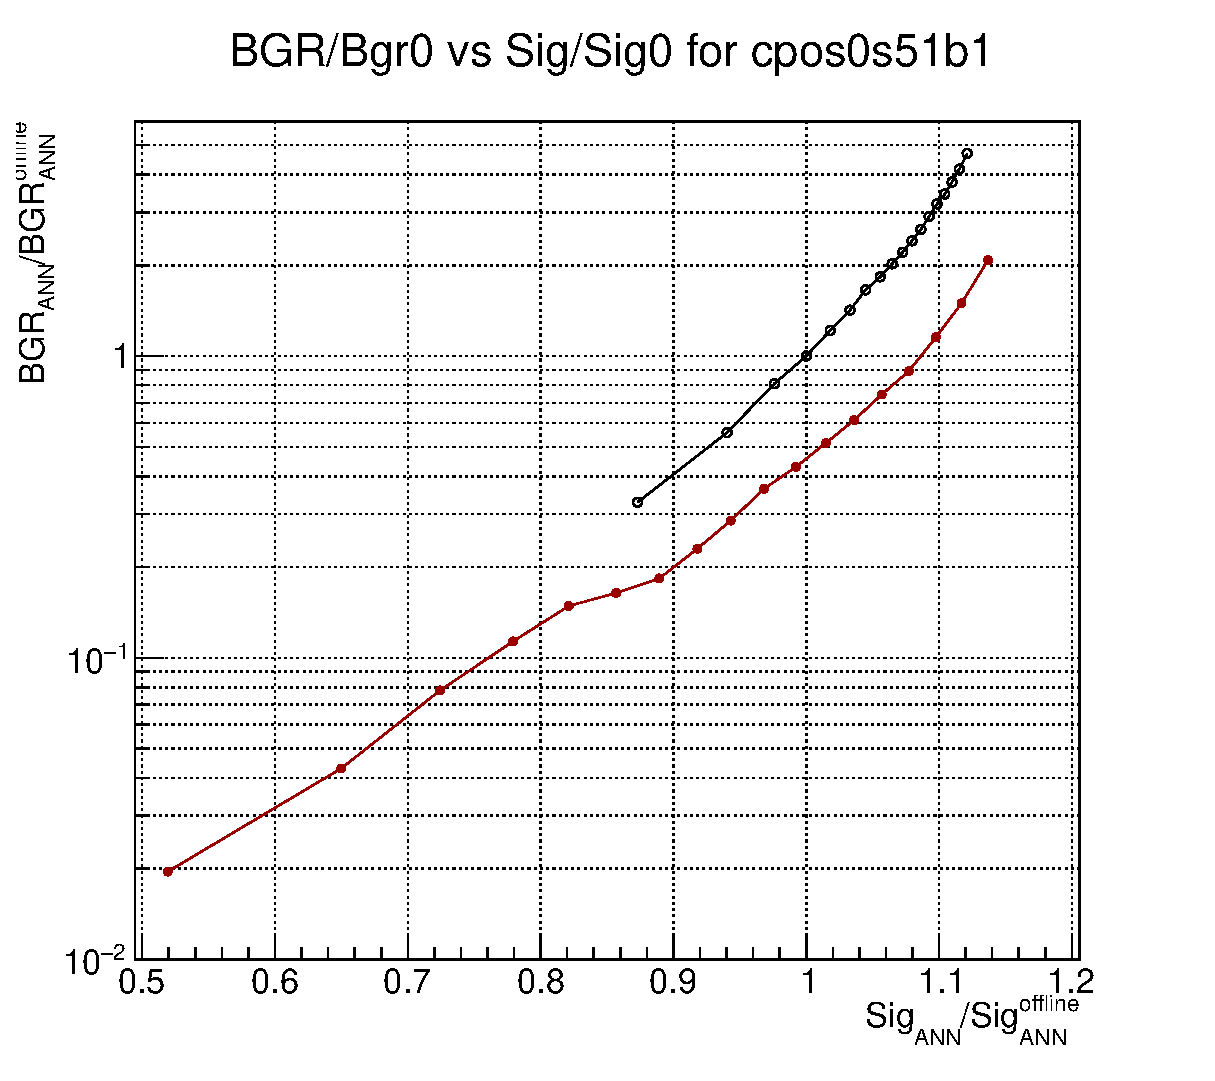
\includegraphics[width=0.55\textwidth]{figures/pdf/mumep_trq_ann_signal_vs_background_log}
      % }
    };
    \node [text width=1cm, scale=1.0] at (13.,3.5) {(b)};
  \end{tikzpicture}
  % \captionof{figure} {
  \caption{
    \label{fig:mumep_trq_ann} 
    DAR (Circles) vs PAR (squares) background vs track selection efficiency.
    Signal: {\bf cpos0s51b1} , signal window {\blue efficiency}, background:{\bf cpos0s51b1} , tracks with $\Delta{P} > 1.0$ MeV.
    Both signal and background are measured in units of signal and background {\blue efficiency} corresponding to the selection
    using {\blue the} default Offline v9\_0\_5 ANN-based track selection, $S_{PAR}^+ > 0.8$.
    {\blue Remove fpos dataset from legend or clarify this is the training dataset}
  }
\end{figure}

%%%%%%%%%%%%%%%%%%%%%%%%%%%%%%%%%%%%%%%%%%%%%%%%%%%%%%%%%%%%%%%%%%%%%%%%%%%%%%
\subsection{Testing charge symmetry of the ANN-based track selection}

It is worth noting that the track parameters used for ANN training \strike{don't} {\blue do not} depend explicitly
on the reconstructed track sign. One could therefore expect the efficiency of the ANN-based
track selection to be charge-symmetric. To check this hypothesis, Figure \ref{fig:su2020_mva_test_dar}
compares {\blue the} efficiency of the {\blue electron trained }ANN-based selection for 105 MeV electrons and 105 MeV positrons
\strike{, where in both cases the tracks were selected with the ANN trained on negative tracks}.

Figure \ref{fig:su2020_mva_test_dar} confirms that for the same track momentum, the ANN-based selection
is charge-symmetric with an accuracy better than 0.5\%.
\strike{\textbackslash n}
The third, and the only visible{\blue , distribution} in Figure \ref{fig:su2020_mva_test_dar} \strike{distribution} corresponds to
\strike{selection of} 105 MeV electron tracks {\blue selected} using {\blue the} ANN trained on 92 MeV positrons as described in
Section \ref{sec:mumep_channel}. One \strike{can} {\blue would} expect {\blue the} efficiency of this selection to be sub-optimal,
{\blue but} rather surprisingly, {\blue the} efficiency is reduced by less than 4\%.
\strike{\textbackslash n}
Observed charge symmetry allows to use one common ANN to select tracks in all channels in {\blue the} \MuToEm\ search 
and another one \strike{-} for track selection in all channels in {\blue the} \MuToEp\ analysis.

\begin{figure}
  % \hspace{-0.6in}
  \begin{tikzpicture}
    \node[anchor=south west,inner sep=0] at (0,0.) {
      % \node[shift={(0 cm,0.cm)},inner sep=0,rotate={90}] at (0,0) {}
      \makebox[\textwidth][c] {
        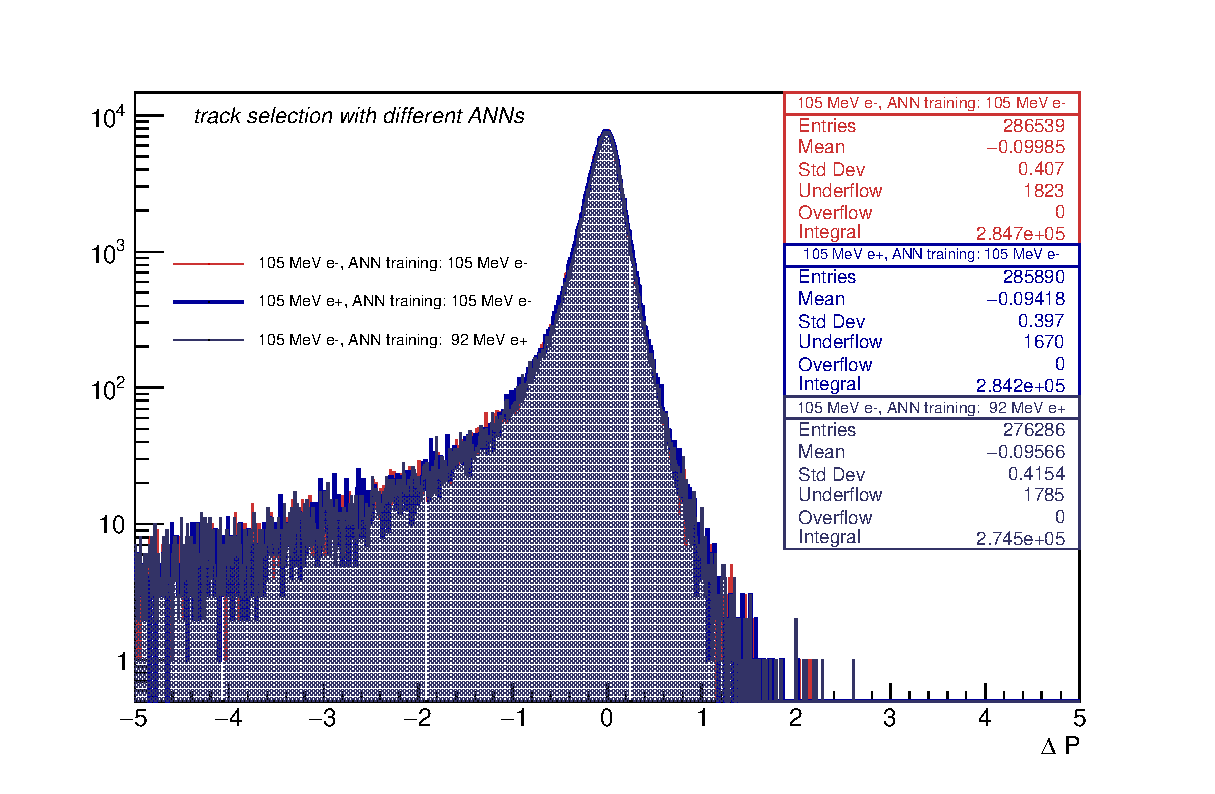
\includegraphics[width=0.95\textwidth]{figures/pdf/figure_00231_su2020_mva_test_dar}
      }
    };
    % \node [text width=6cm, scale=0.8] at (4.5,6.4) {mu2e-18894 by Kevin Lynch and Jim Popp};
  \end{tikzpicture}
  % \captionof{figure} {
  \caption{
    \label{fig:su2020_mva_test_dar} 
    \strike{Electron and positron selection, 105 MeV , positron selection - 90 MeV/c}
    {\blue 105 MeV/c electrons and positrons selected using 105 MeV/c electron, 105 MeV/c positron,
      and 92 MeV/c positron trained ANNs.}
    {\blue Legend should be clearer on generated particle/ANN. Perhaps: 105 MeV/c electrons using 92 MeV/c positron trained ANN?}
  }
\end{figure}


%%%%%%%%%%%%%%%%%%%%%%%%%%%%%%%%%%%%%%%%%%%%%%%%%%%%%%%%%%%%%%%%%%%%%%%%%%%%%%
\subsection{Track selection cuts summary}
\label{sec:track-selection_cuts_summary}
  
For SU2020 analyses, a well reconstructed track is a DAR track satisfying the following requirements {\blue :}

\begin{itemize}
\item
  the track impact parameter, $D0$, is consistent with the track coming from the stopping target: 
  $|D0| < 100$ mm. We note that $D0$ is calculated at the point of the reconstructed trajectory 
  inside the Mu2e tracker {\blue which point inside the tracker?}, several meters away from the stopping target,
  and {\blue therefore} cannot be directly compared with the radius of the stopping target foils
\item 
  the track dip angle, $\lambda = 90^o - \alpha$, where $\alpha$ is the track angle with respect 
  to the solenoid axis, is within $ 0.5 < \tan{\lambda} < 1$. 
  The choice of the lower cutoff value, 0.5, is not currently dictated by any real considerations.
  It is a clean-up cutoff, which \strike{doesn't} {\blue does not} introduce any visible inefficiency. 
  The requirement $\tan{\lambda} < 1$ reduces the tracking acceptance by about 10\%, 
  and, most importantly, is an anti-cosmics selection. This cut also rejects tracks of particles 
  produced upstream of the stopping target, i.e. coming from the TS
\item
  track quality ANN score $S_{ANN} > 0.2$ {\blue .}
\end{itemize}

Although {\blue the} \MuToEm\ and \MuToEp\ analyses use different track quality ANN's trained using tracks in {\blue a} different
momentum range, the cut value \strike{ison} {\blue on} the ANN score \strike{isthe} {\blue is the} same in both cases.
It \strike{was} verifies that the ANN-based track selection is charge-symmetric, i.e. for a given momentum,
the track selection efficiency \strike{doesn't} {\blue does not} depend on the reconstructed track charge.
